
%\begin{figure}[H]
%     \centering
%     \includegraphics[width=1.0\textwidth]{figure/appendix/XceptionNet}
%     \caption{The whole architecture of XceptionNet used in our experiment.} %\label{fig18}
%\end{figure}

\section{Suricata Detection Rules}

The Suricata detection rules used in this study are provided in Listing~\ref{lst:suricata_local_rules}. These rules define the packet-level detection logic for the selected Modbus TCP attack scenarios, including device fingerprinting, protocol fuzzing, unauthorized write commands, diagnostic command injection, and TCP SYN flooding.
\newpage

\lstinputlisting[style=appendixcode,caption={Suricata detection rules defined in the local.rules file},label={lst:suricata_local_rules}]{code/local.rules}
\newpage

\section{Graylog Alert Rules for Attack Scenario Detection}

This section lists the Graylog alert rules configured for detecting the eight
attack scenarios evaluated in this study. Each rule corresponds to a specific
attack behavior and was used to validate the detection capability of the
proposed monitoring framework.

\subsection{Scenario A - Reconnaissance Scanning}
\begin{figure}[htbp]
\centering
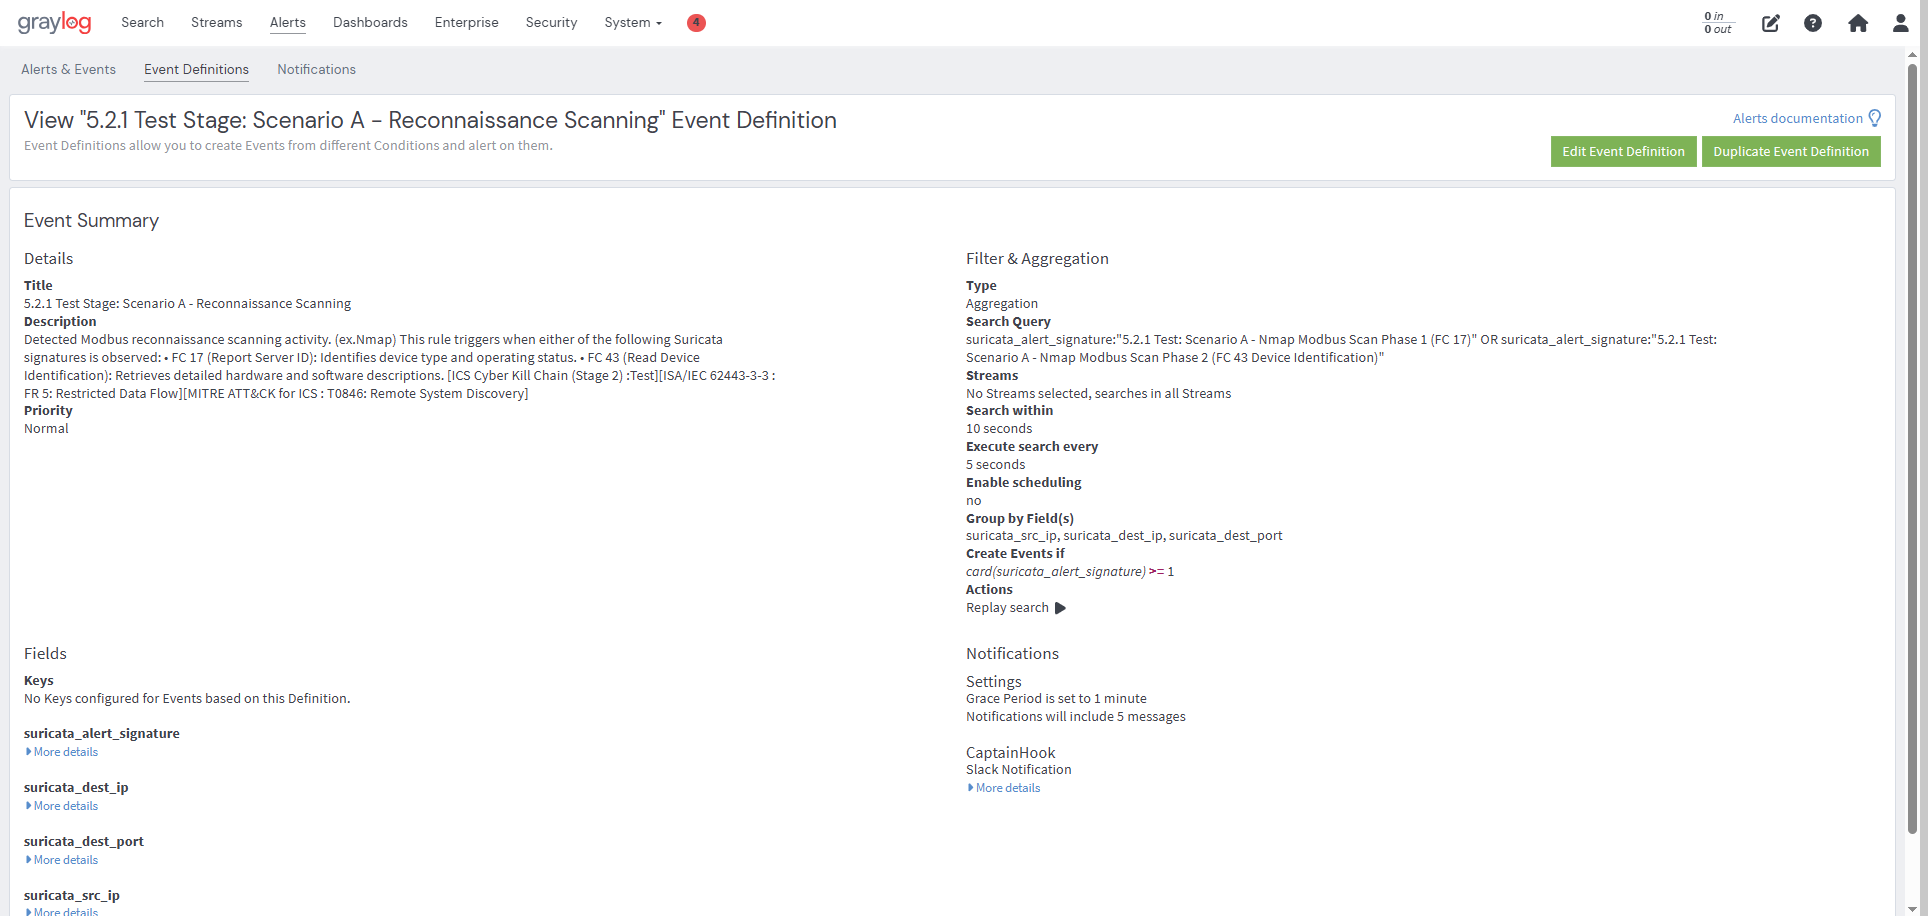
\includegraphics[width=15.5cm]{figure/Figure_A.2.1.Graylog-5.2.1 Event Definition.png}
\caption{Scenario A - Reconnaissance Scanning} 
\end{figure}
\newpage

\subsection{Scenario B1 - Request-side Modbus Protocol Probing}
\begin{figure}[htbp]
\centering
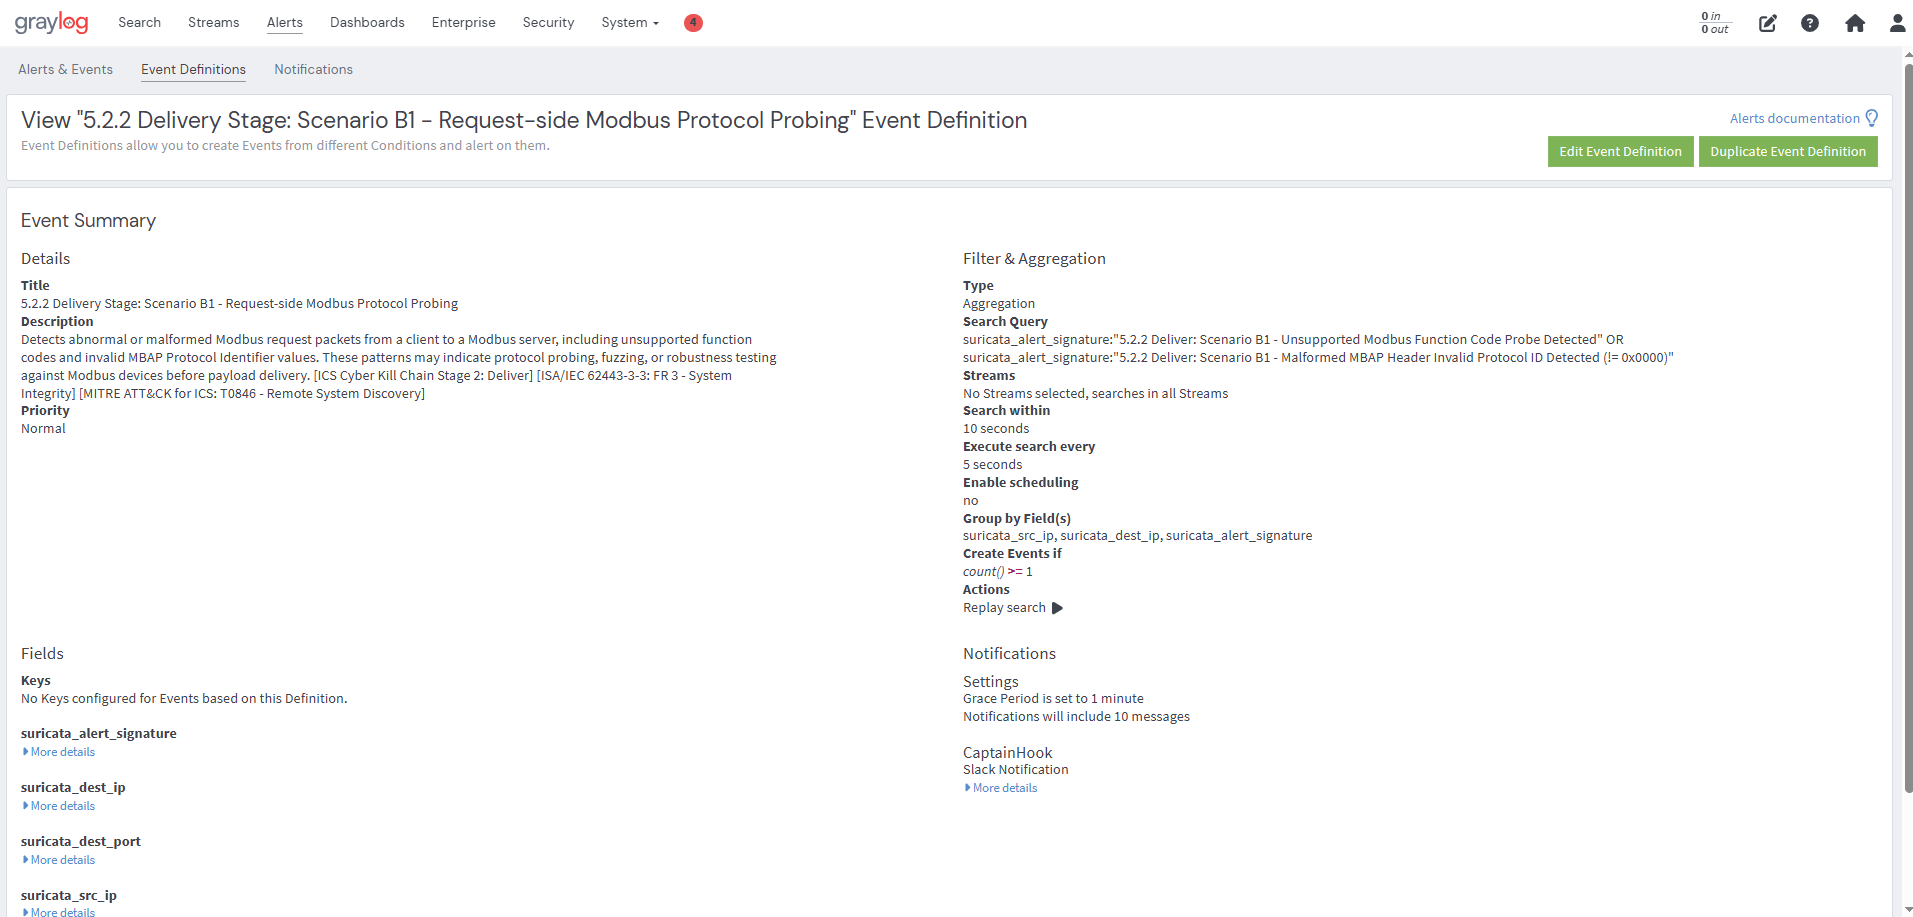
\includegraphics[width=15.5cm]{figure/Figure_A.2.2.Graylog-5.2.2 Event Definition.png}
\caption{Scenario B1 - Request-side Modbus Protocol Probing} 
\end{figure}
\newpage

\subsection{Scenario B2 - Response-side Modbus Exception Detection}
\begin{figure}[htbp]
\centering
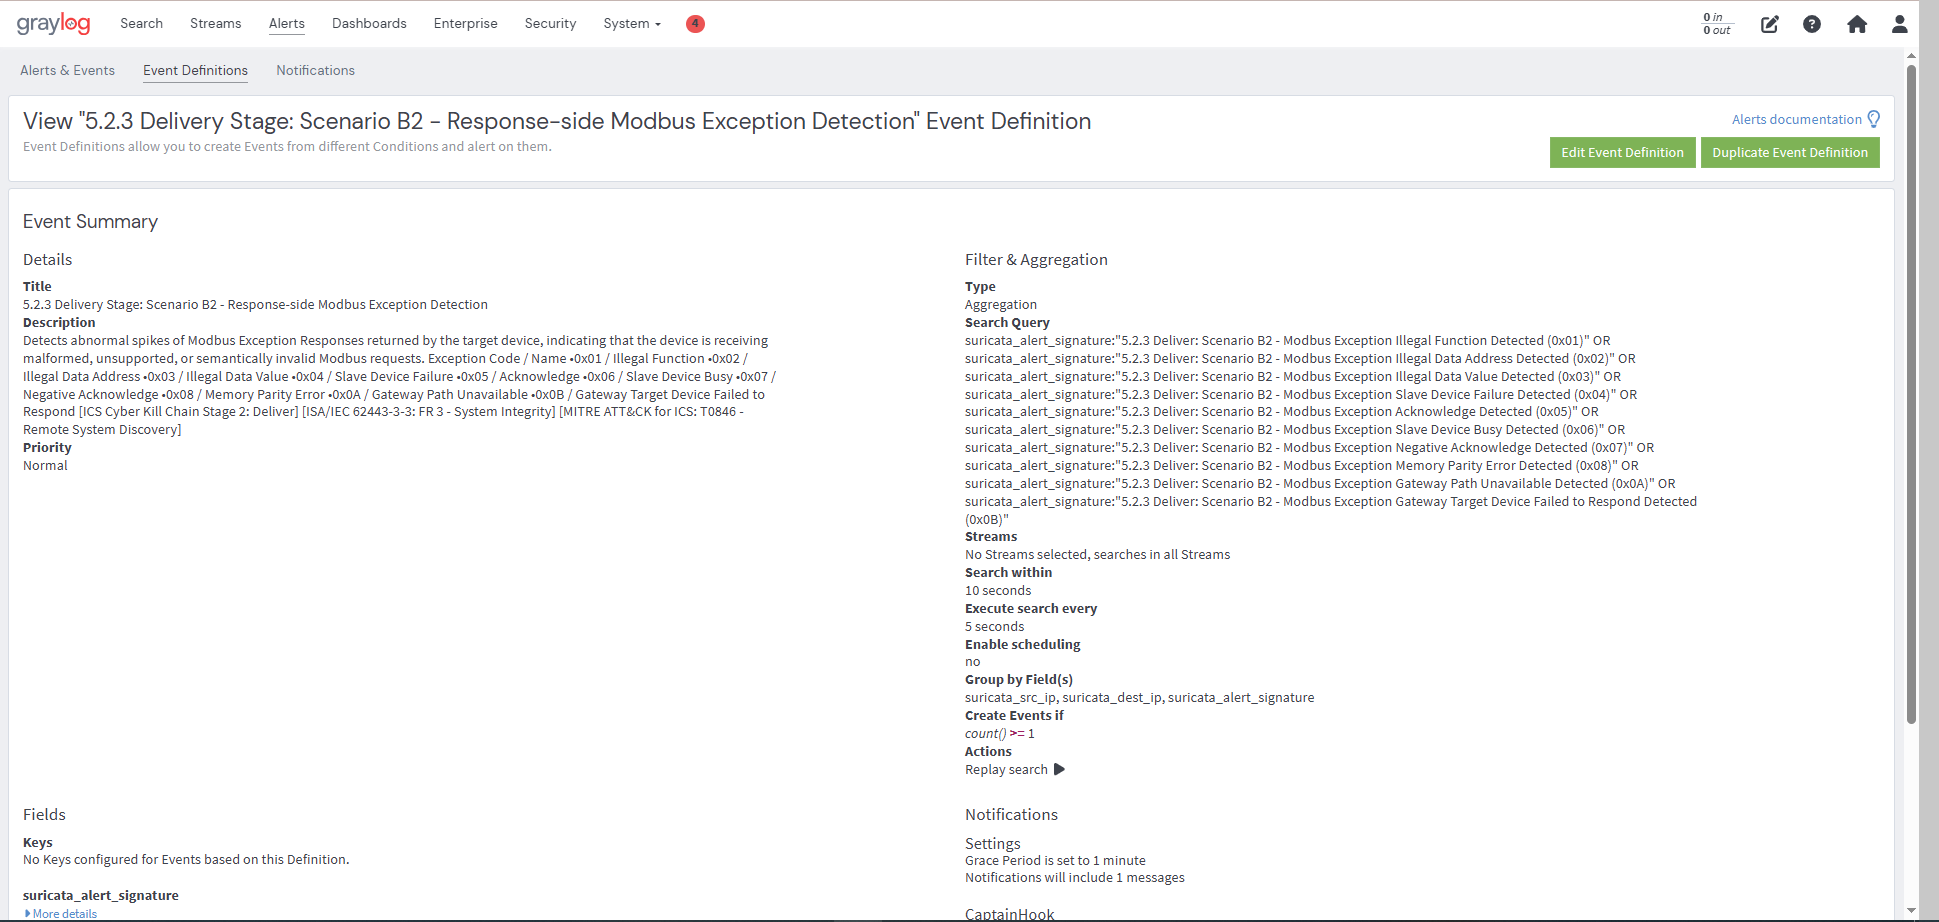
\includegraphics[width=15.5cm]{figure/Figure_A.2.3.Graylog-5.2.3 Event Definition.png}
\caption{Scenario B2 - Response-side Modbus Exception} 
\end{figure}
\newpage

\subsection{Scenario C1 - Unauthorized Modification}
\begin{figure}[htbp]
\centering
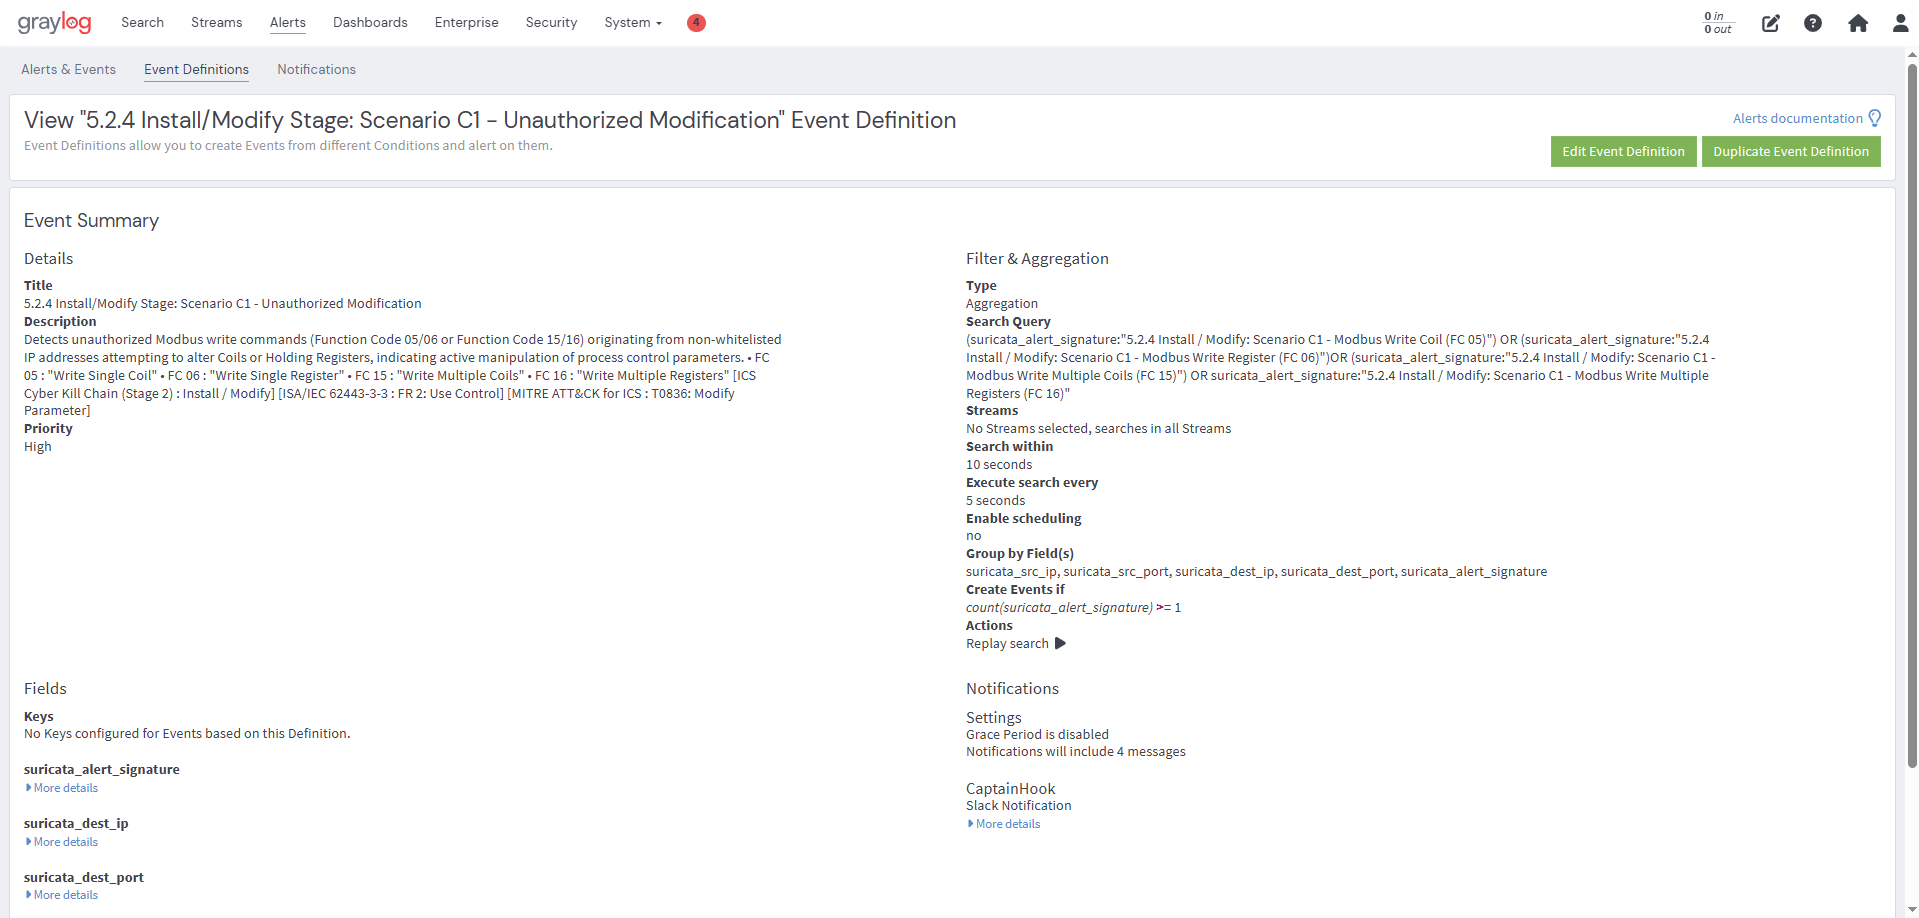
\includegraphics[width=15.5cm]{figure/Figure_A.2.4.Graylog-5.2.4 Event Definition.png}
\caption{Scenario C1 - Unauthorized Modification} 
\end{figure}
\newpage

\subsection{Scenario C2 - Advanced Register Manipulation}
\begin{figure}[htbp]
\centering
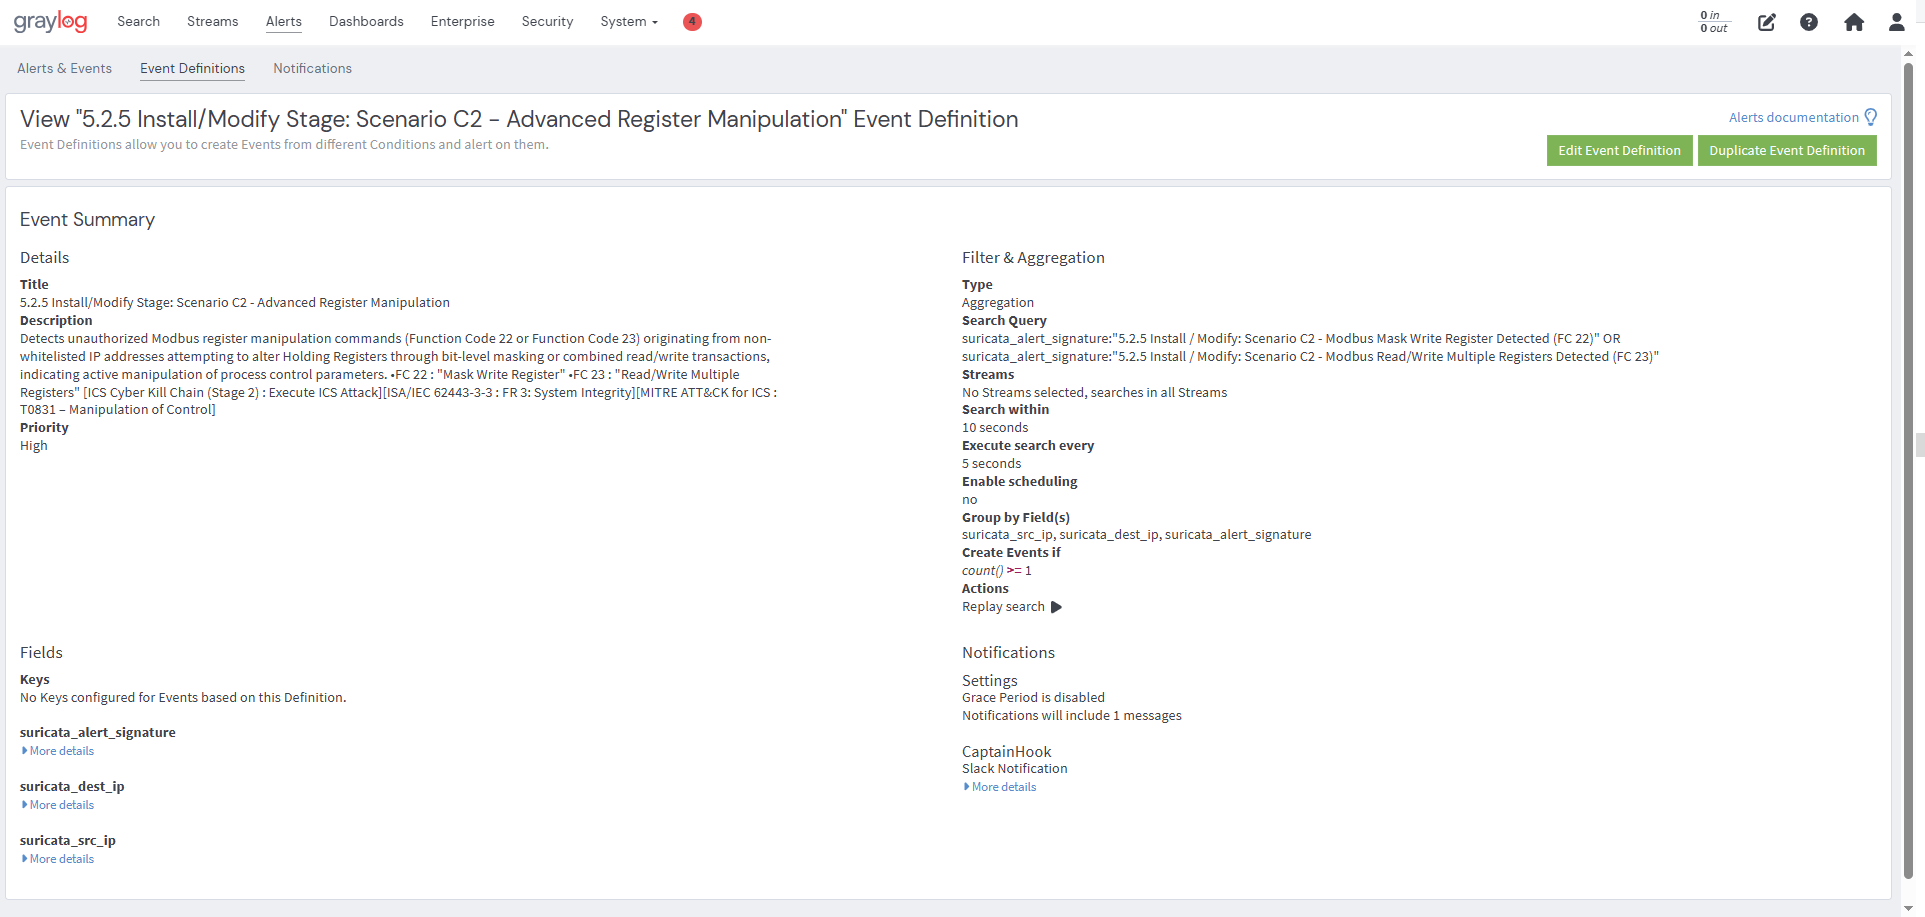
\includegraphics[width=15.5cm]{figure/Figure_A.2.5.Graylog-5.2.5 Event Definition.png}
\caption{Scenario C2 - Advanced Register Manipulation} 
\end{figure}
\newpage

\subsection{Scenario D - Critical Diagnostic Command Injection}
\begin{figure}[htbp]
\centering
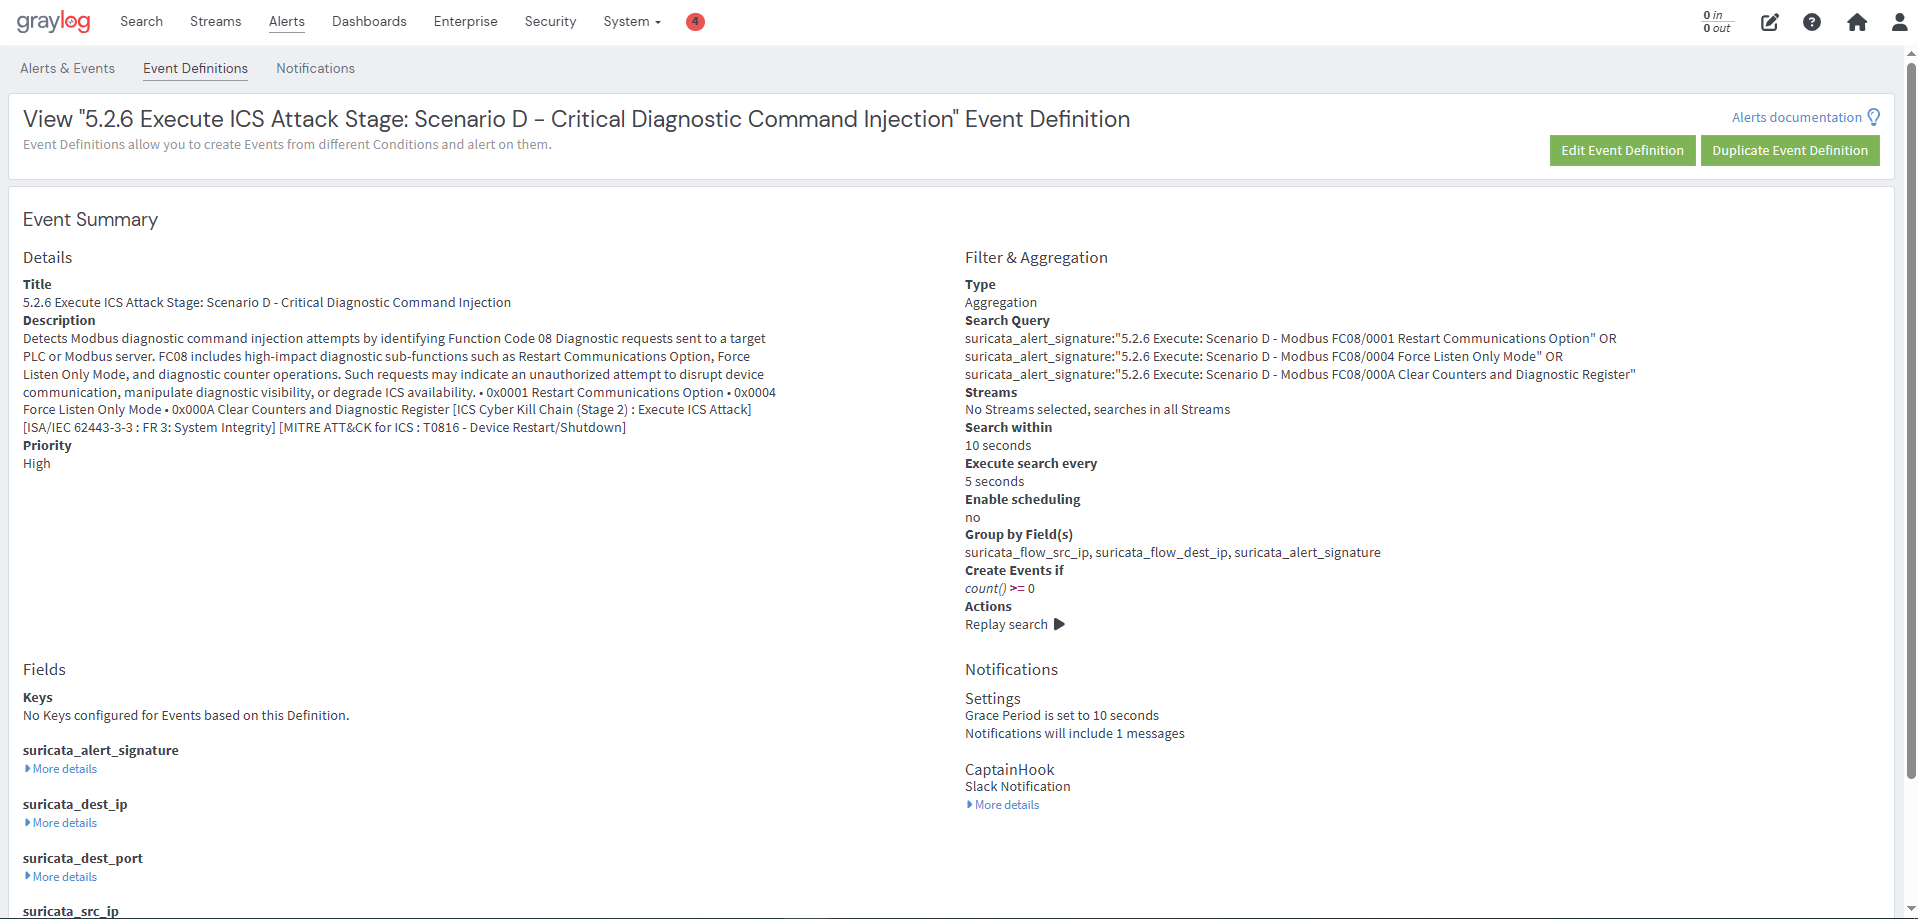
\includegraphics[width=15.5cm]{figure/Figure_A.2.6.Graylog-5.2.6 Event Definition.png}
\caption{Scenario D - Critical Diagnostic Command Injection} 
\end{figure}
\newpage

\subsection{Scenario E1 - Modbus TCP/502 High-rate SYN Activity}
\begin{figure}[htbp]
\centering
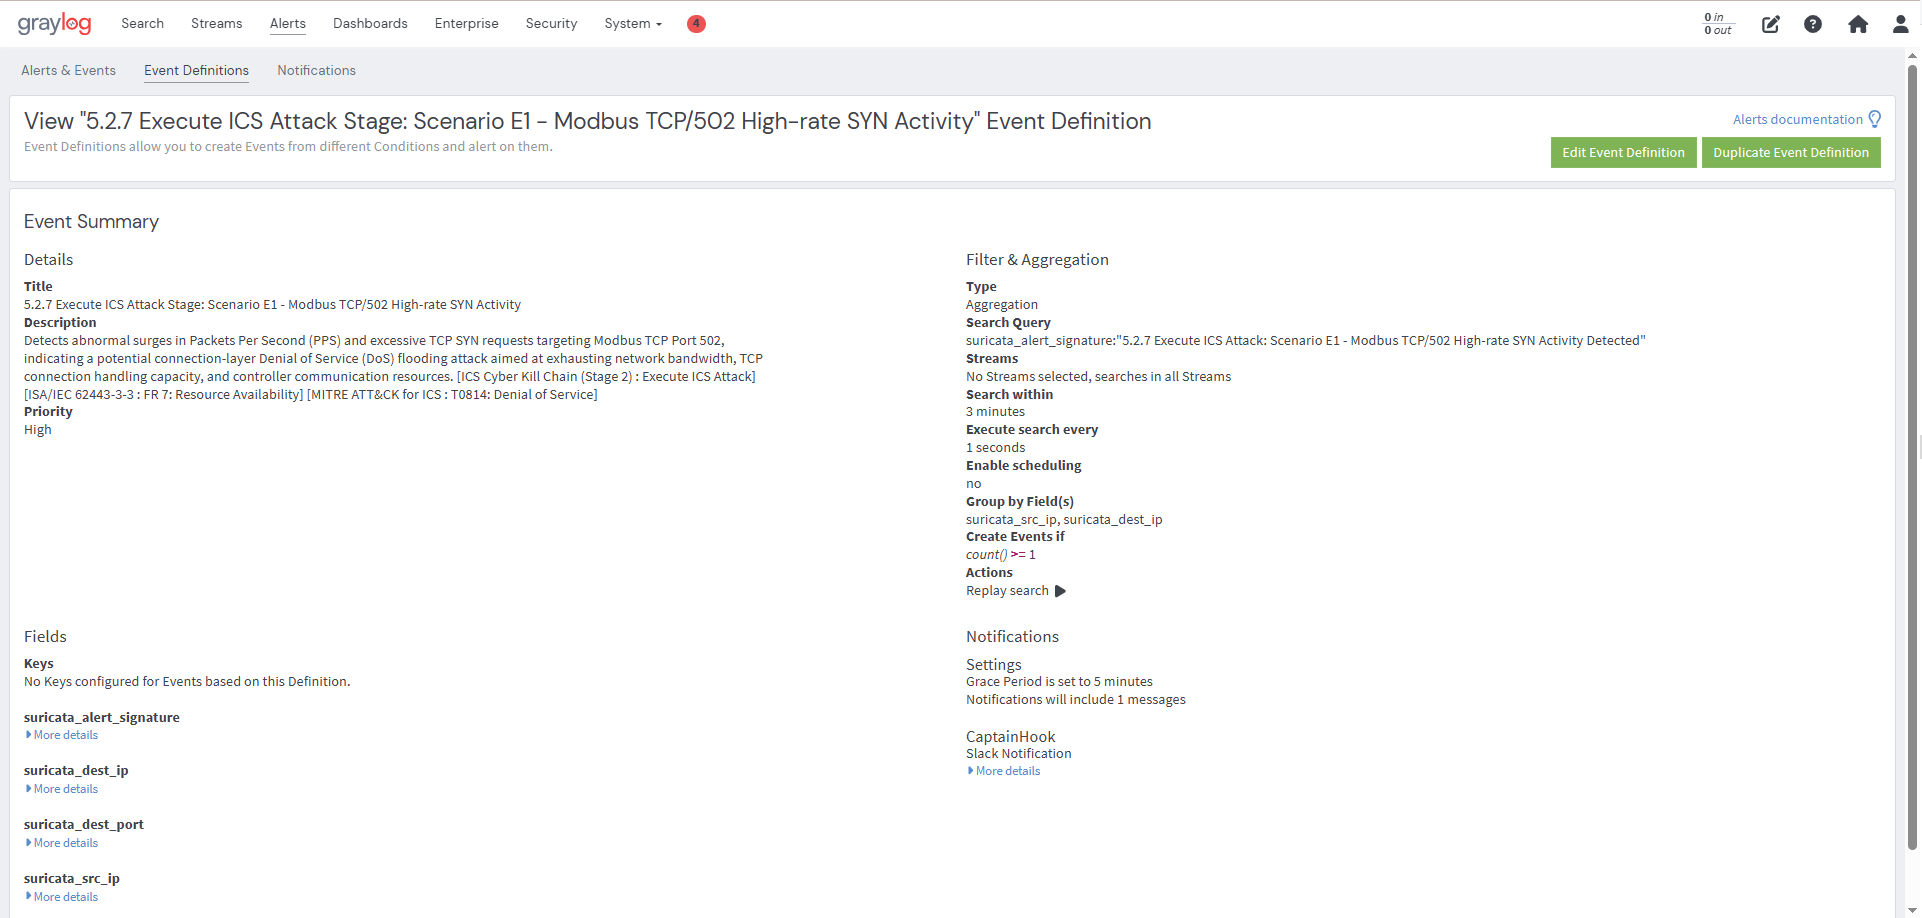
\includegraphics[width=15.5cm]{figure/Figure_A.2.7.Graylog-5.2.7 Event Definition.png}
\caption{Scenario E1 - Modbus TCP/502 High-rate SYN Activity} 
\end{figure}
\newpage

\subsection{Scenario E2 - Modbus TCP/502 High-rate Payload Activity}
\begin{figure}[htbp]
\centering
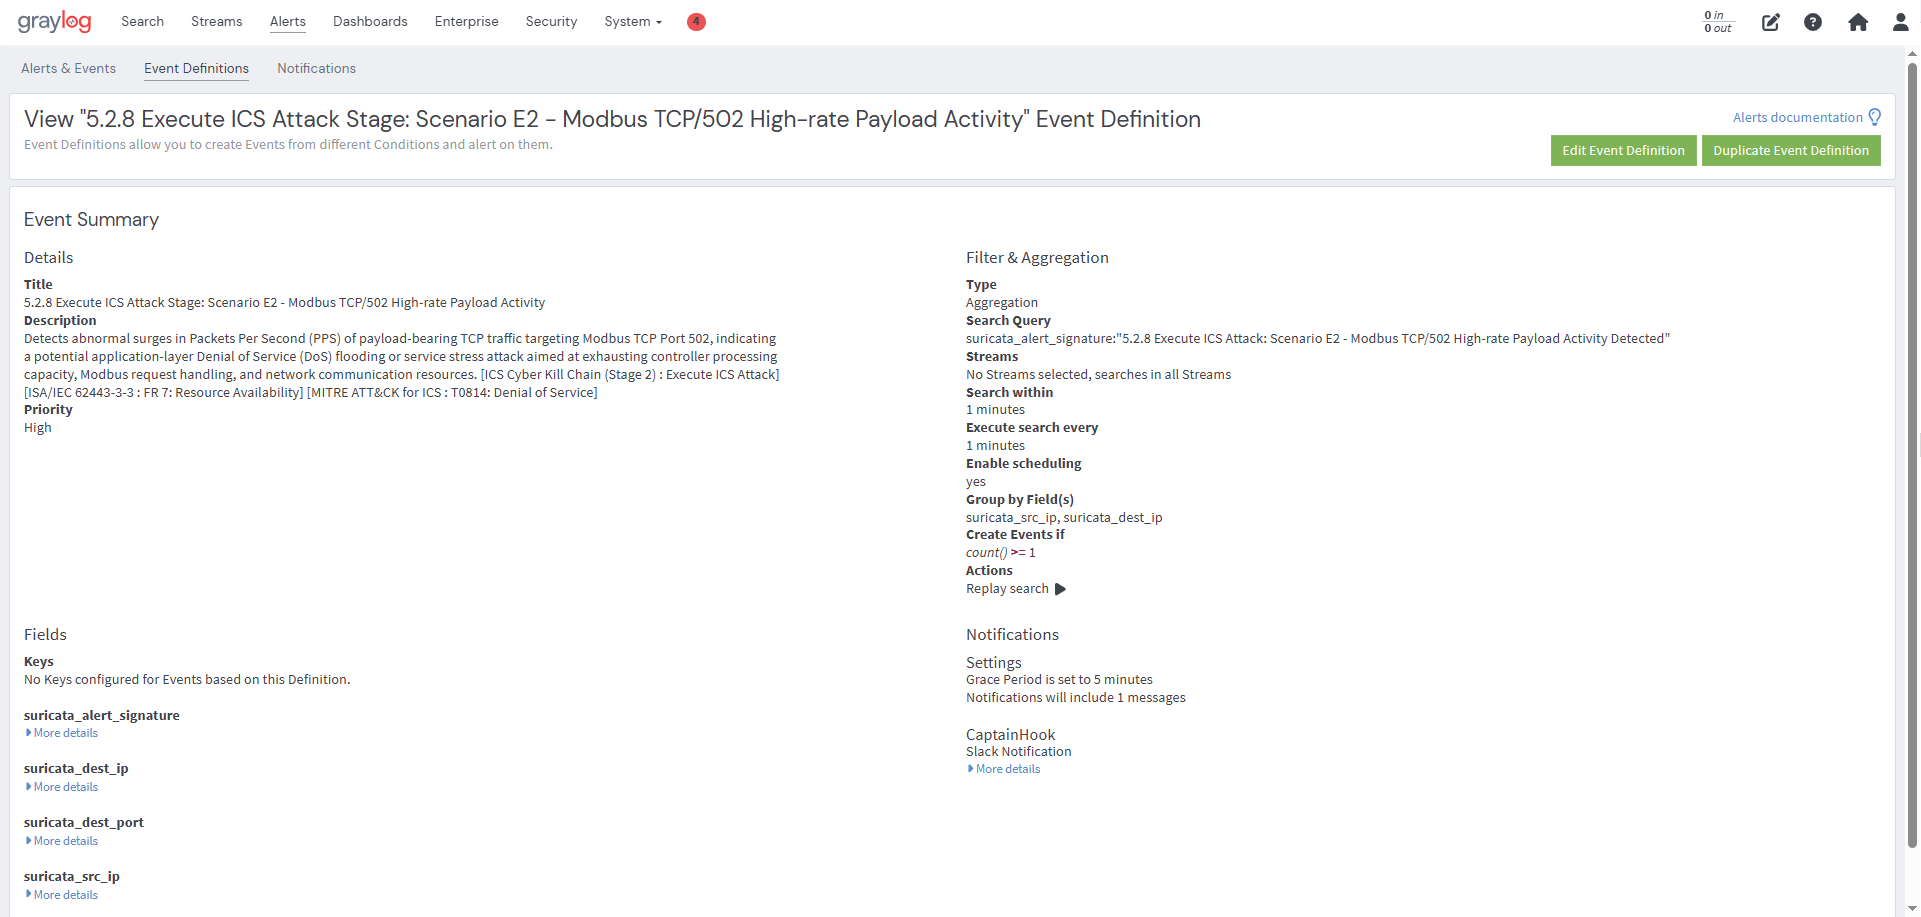
\includegraphics[width=15.5cm]{figure/Figure_A.2.8.Graylog-5.2.8 Event Definition.png}
\caption{Scenario E2 - Modbus TCP/502 High-rate Payload Activity} 
\end{figure}
\newpage

\section{Baseline Modbus Traffic Generation Script}
\label{sec:baseline-modbus-script}

This script generates baseline Modbus TCP read traffic for comparison with malicious and fuzzing activities.

\lstinputlisting[
    language=Python,
    caption={Baseline Modbus TCP Traffic Generation Script},
    label={lst:baseline-modbus-traffic}
]{code/baseline_modbus_traffic.py}
\newpage

\section{Attack Payloads}
The following attack scripts were used to validate the attack scenarios presented
in this paper, covering Scenarios B1 (Listing~\ref{lst:scenario-b1}),
B2 (Listing~\ref{lst:scenario-b2}),C1 (Listing~\ref{lst:scenario-c1}),C2 (Listing~\ref{lst:scenario-c2}),D (Listing~\ref{lst:scenario-d}), and E2 (Listing~\ref{lst:scenario-e2}).

\subsection{Scenario B1: Request-side Modbus Protocol Probing}
\lstinputlisting[
  language=python,
  caption={Scenario B1: Request-side Modbus Protocol Probing},
  label={lst:scenario-b1}
]{code/Scenario-B1.py}

\subsection{Scenario B2: Response-side Modbus Exception}
\lstinputlisting[
  language=python,
  caption={Scenario B2: Response-side Modbus Exception},
  label={lst:scenario-b2}
]{code/Scenario-B2-Client.py}

\subsection{Scenario C1: Unauthorized Modification}
\lstinputlisting[
  language=python,
  caption={Scenario C1: Unauthorized Modification},
  label={lst:scenario-c1}
]{code/Scenario-C1.py}

\subsection{Scenario C2: Advanced Register Manipulation}
\lstinputlisting[
  language=python,
  caption={Scenario C2: Advanced Register Manipulation},
  label={lst:scenario-c2}
]{code/Scenario-C2.py}

\subsection{Scenario D: Critical Diagnostic Command Injection}
\lstinputlisting[
  language=python,
  caption={Scenario D: Critical Diagnostic Command Injection},
  label={lst:scenario-d}
]{code/Scenario-D.py}

\subsection{Scenario E2: Modbus TCP/502 High-rate Payload Activity}
\lstinputlisting[
  language=python,
  caption={Scenario E2: Modbus TCP/502 High-rate Payload Activity},
  label={lst:scenario-e2}
]{code/Scenario-E2.py}